\begin{spacing}{1}
  \chapter*{Abstract}
\end{spacing}
\begin{wrapfigure}{r}{0.3\textwidth}
  \begin{center}
    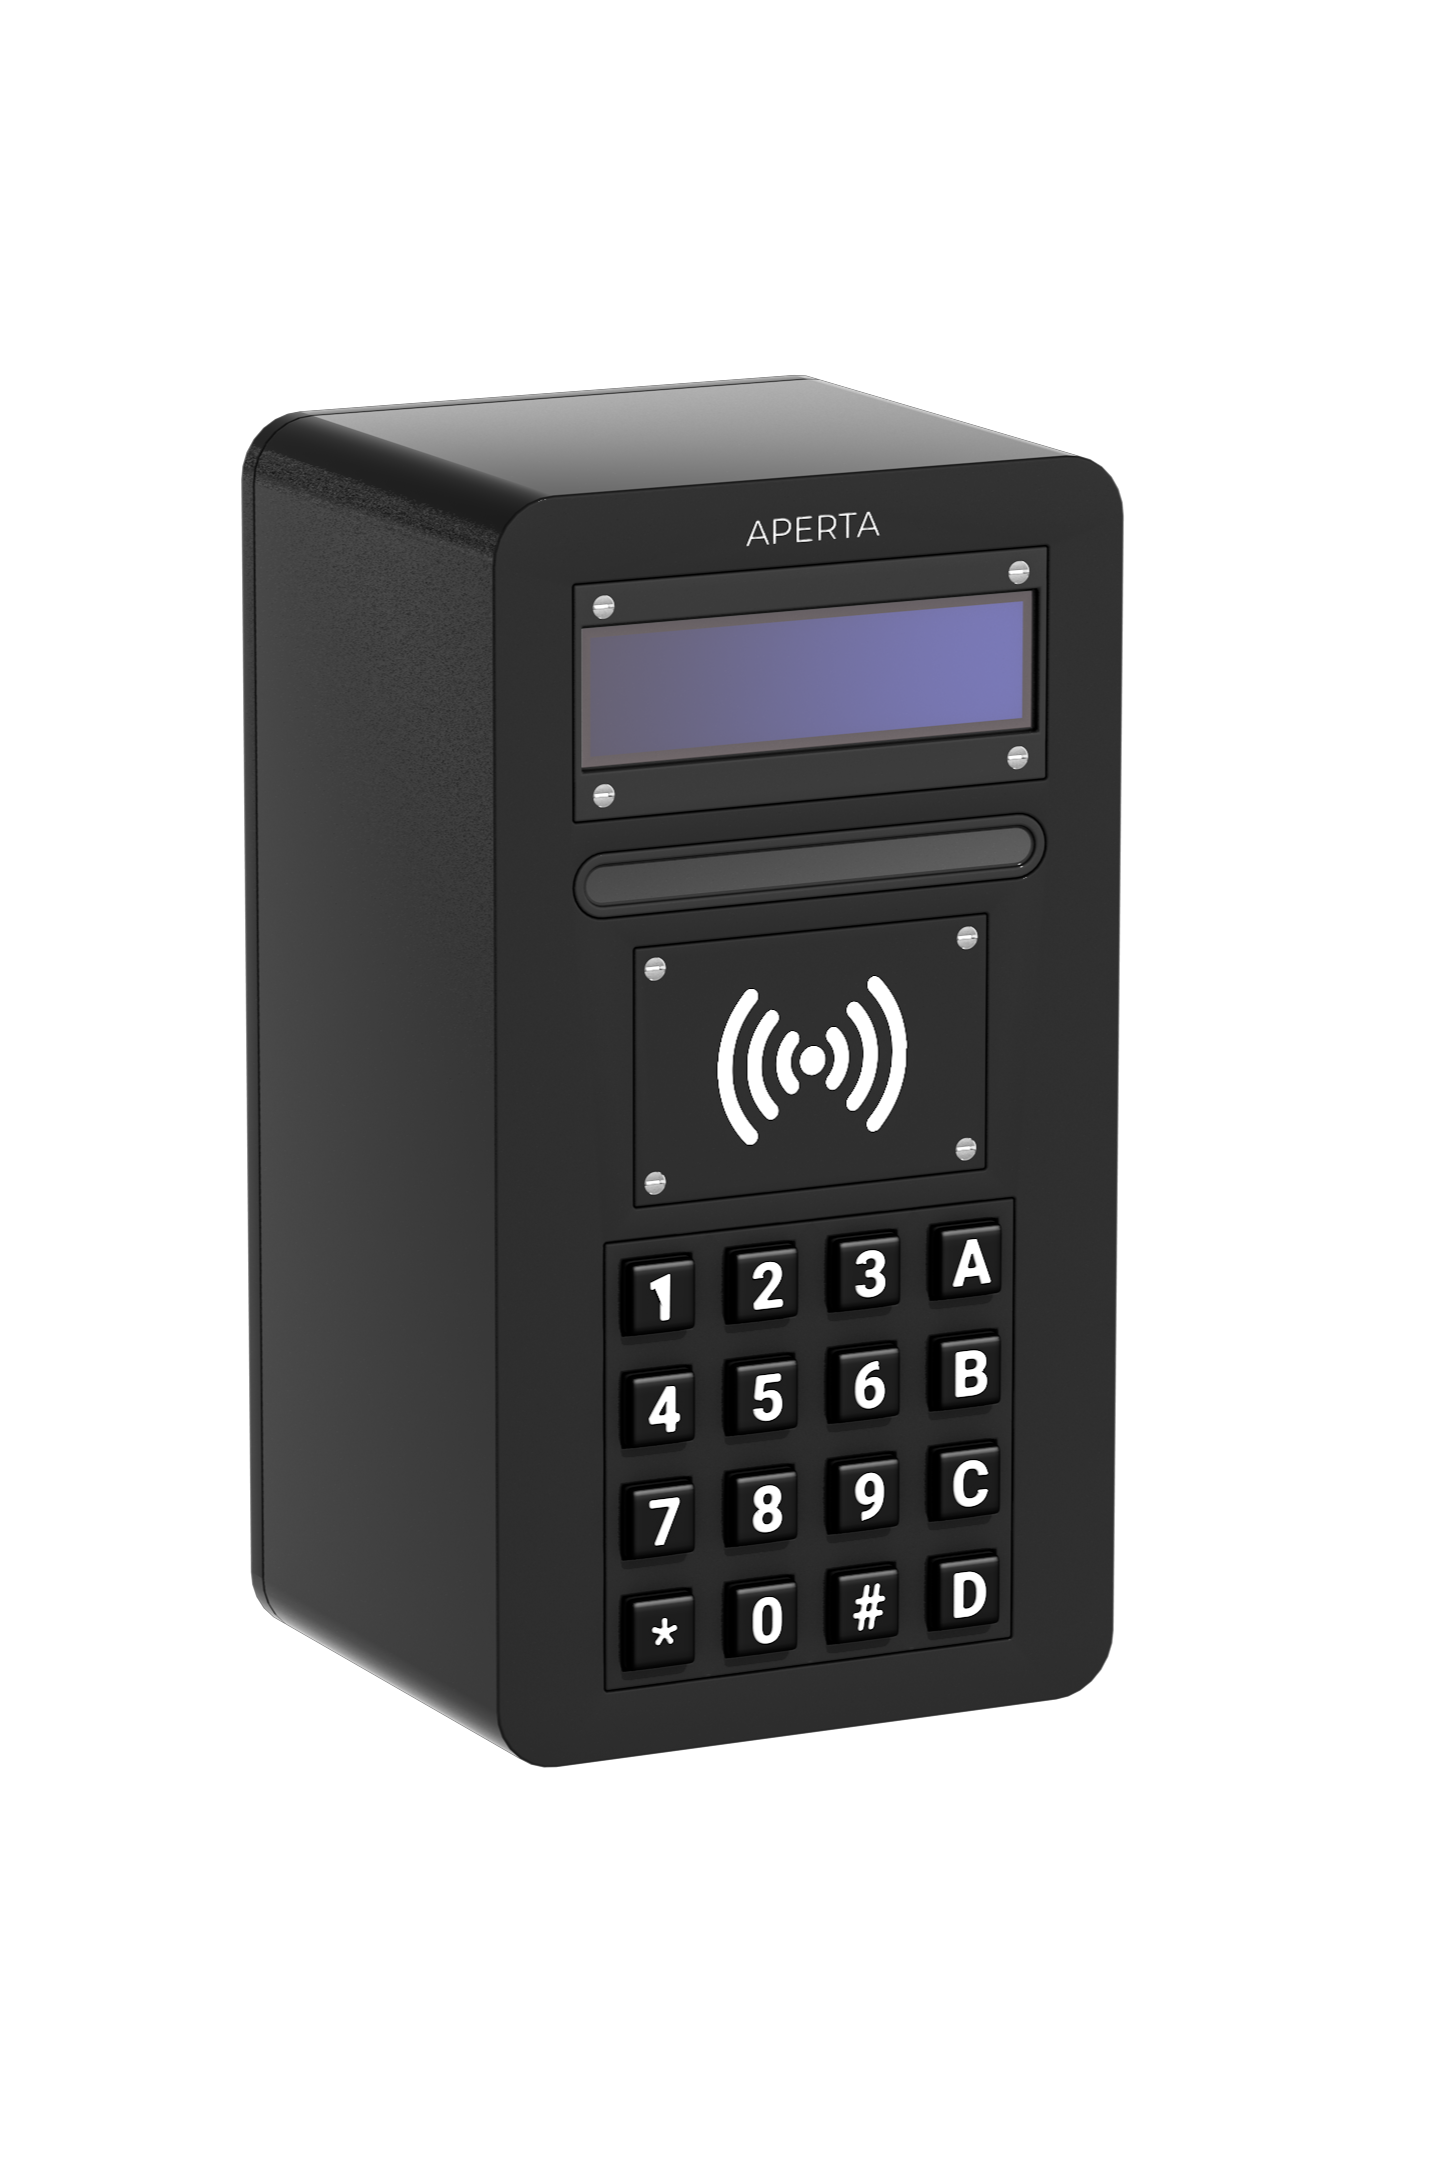
\includegraphics[width=0.5\textwidth]{pics/all-in-package.png}
    \caption{Rendered Prototyp}
  \end{center}
\end{wrapfigure}
APERTA is a garage door system that was developed by Benjamin Golic, David Hauser and Simon Koll as part of their diploma thesis. The system can be retrofitted to electric garage doors regardless of the manufacturer and enables entry into the world of the Internet of Things, the IOT. Depending on the configuration, the system consists of up to 3 components, each of which represents an access option to the garage. These are a classic numpad, an RFID reader, and a camera, which is used for license plate recognition. In the future, these can be expanded to include other or further authentication options. A web dashboard is used to manage the combinations of the numpad , NFC card details or license plates. These can be provided with a time validity range. There is also an online store where the product can be configured and spare parts or expansion modules can be purchased. The dashboard, which was implemented using Angular, communicates with the Node-JS server as the backend. It acts as the core, passes the information to the MongoDB database and is available for requests from the Raspberry Pi, which is responsible for the hardware.

\newpage
\begin{spacing}{1}
  \chapter*{Zusammenfassung}
\end{spacing}
\begin{wrapfigure}{r}{0.3\textwidth}
  \begin{center}
    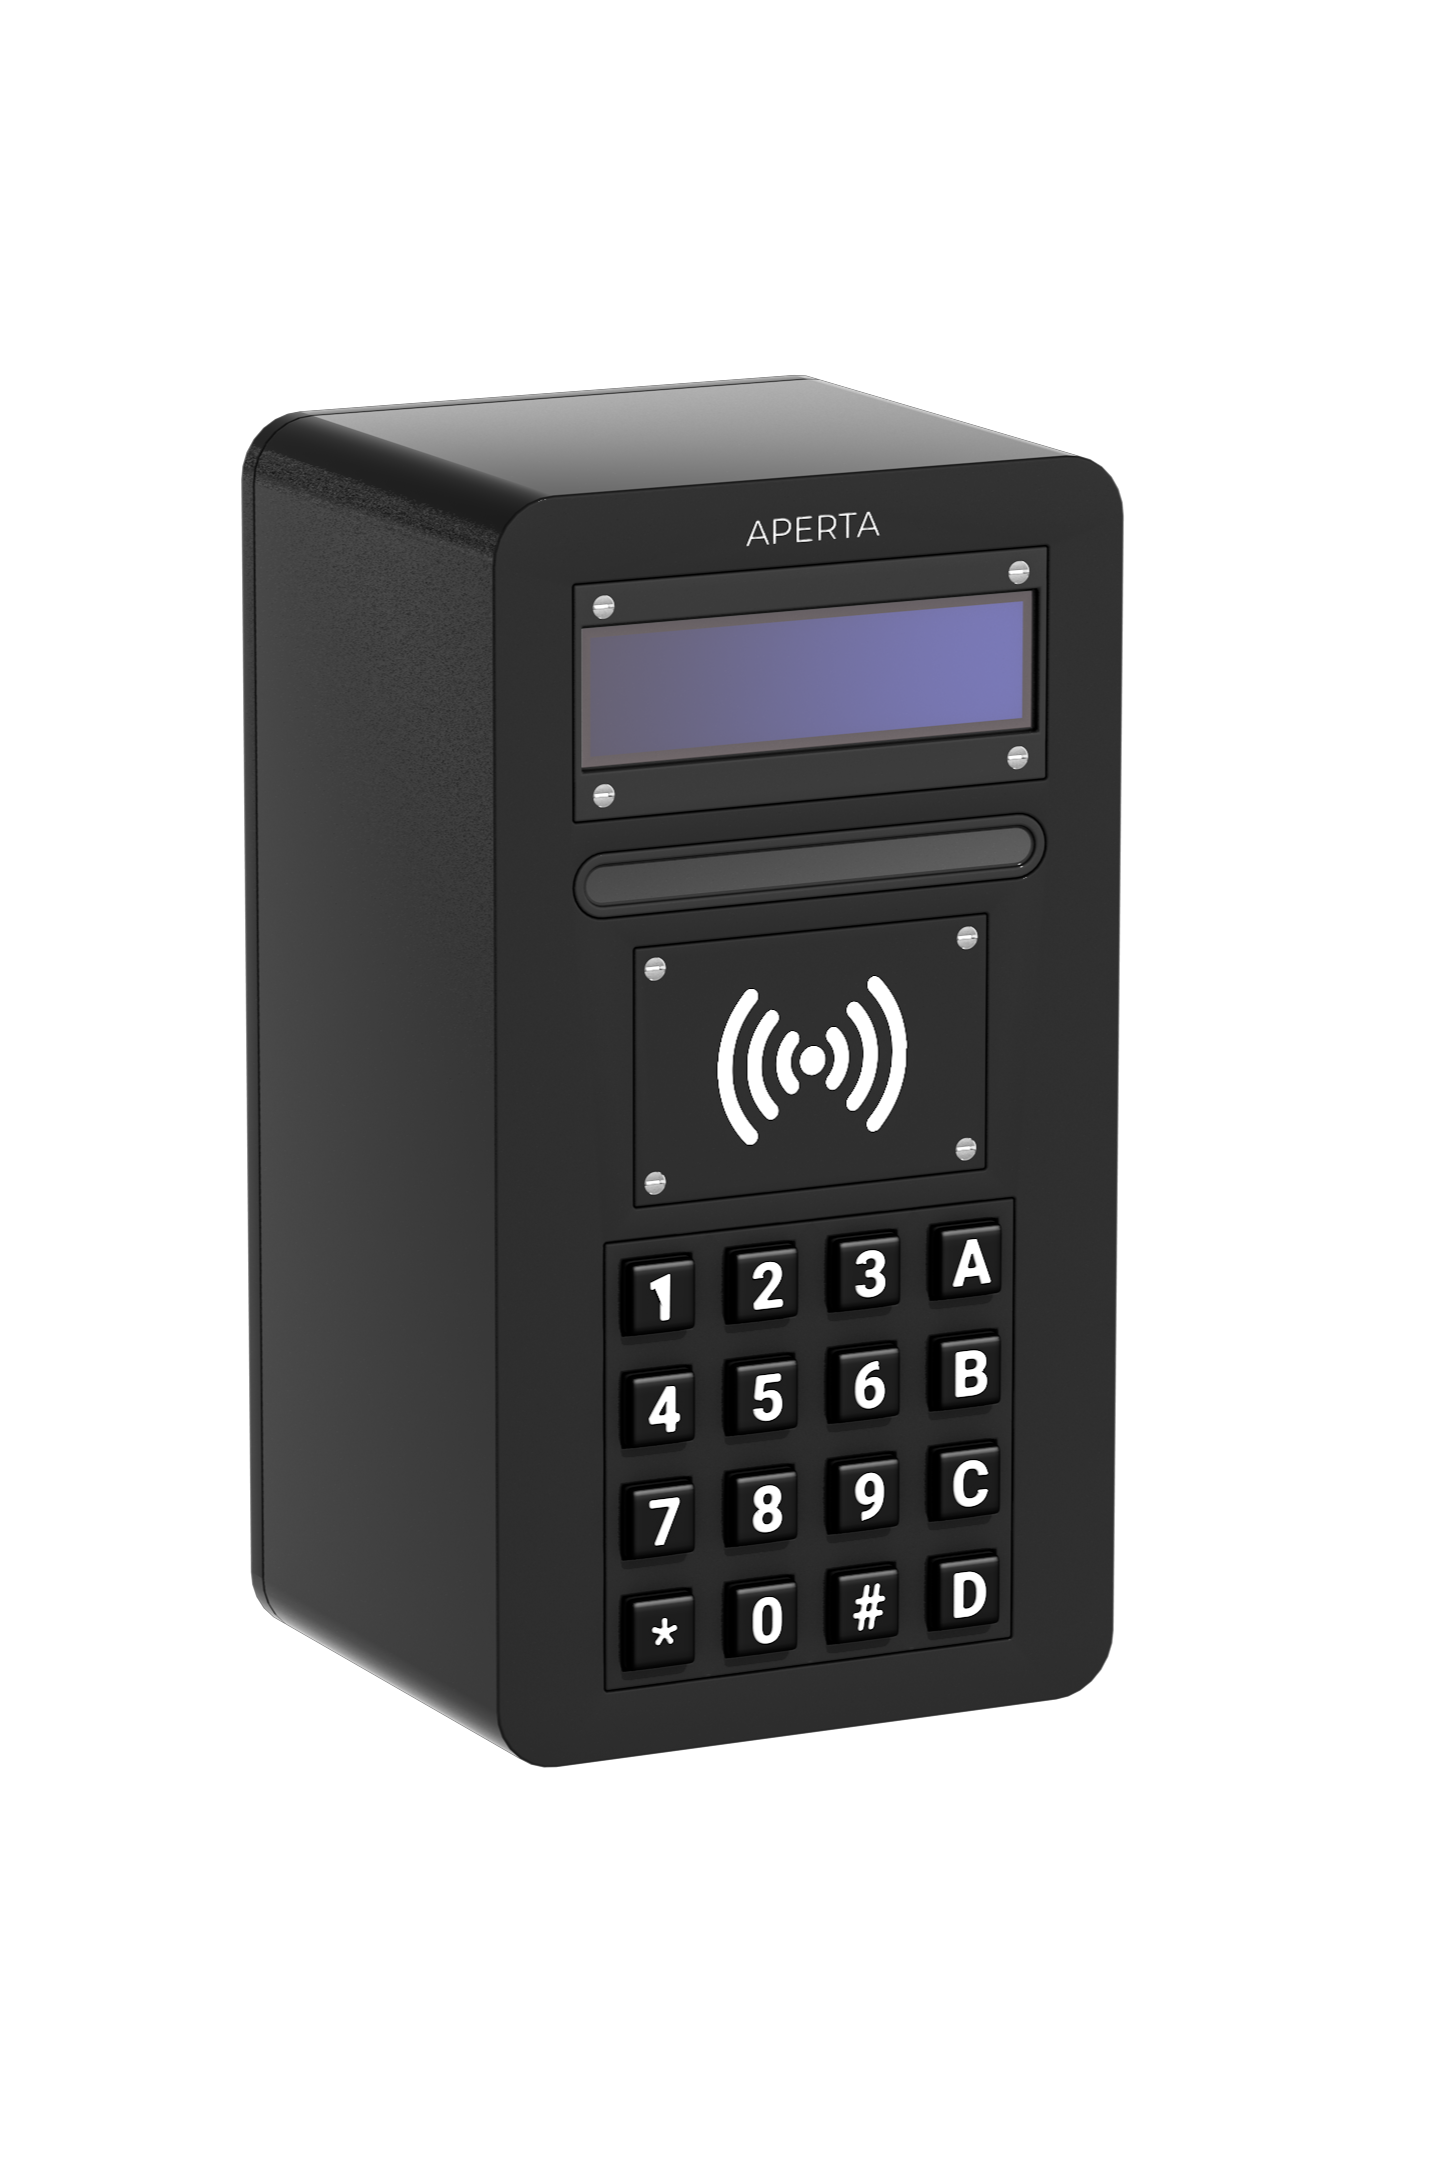
\includegraphics[width=0.5\textwidth]{pics/all-in-package.png}
    \caption{Gerenderter Prototyp}
  \end{center}
\end{wrapfigure}
APERTA ist ein Garagentorsystem, welches von Benjamin Golic, David Hauser und Simon Koll im Rahmen der Diplomarbeit entwickelt wurde. Das System ist herstellerunabhängig bei elektrischen Garagentoren nachrüstbar und ermöglicht den Einstieg in die Welt des Internet der Dinge, dem IOT. Das System besteht, je nach Konfiguration, aus bis zu 3 Komponenten, welche je eine Zutrittsmöglichkeit zur Garage darstellen. Es handelt sich hierbei um ein klassisches Nummernfeld, einem RFID-Lesegerät, und einer Kamera, welche für eine Kennzeichenerkennung genutzt wird. Zukünftig können diese noch um andere oder weitere Möglichkeiten der Authentifizierung erweitert werden. Über ein Web-Dashboard werden die Nummernfeldkombinationen, NFC-Kartendetails oder Kennzeichen verwaltet. Diese können mit einem zeitlichen Gültigkeitsbereich versehen werden. Darüber hinaus gibt es einen Onlineshop, in welchem das Produkt konfiguriert werden kann sowie Ersatzteile oder Erweiterungsmodule erworben werden können. Das Dashboard, welches mithilfe von Angular umgesetzt wurde, kommuniziert mit dem Node-JS Server als Backend. Dieser fungiert als Herzstück und reicht die Informationen an die MongoDB-Datenbank weiter und steht für Anfragen des Raspberry Pi, welcher für die Hardware zuständig ist, zur Verfügung.